% どちらでも確認
\documentclass[10pt]{jarticle} 
% \documentclass[twocolumn,10pt]{jreport}

% 通常パッケージ
\usepackage[top=20truemm,bottom=20truemm,left=20truemm,right=20truemm]{geometry} % 余白設定
\usepackage[dvipdfmx]{graphicx,color} % 図形
\usepackage{otf} % 旧自体

% カスタムパッケージ
\usepackage{listings,jlisting} % ソースをきれいに
\usepackage{url} % URLをきれいに
\usepackage{eclbkbox}  % 文章を枠で囲む
\usepackage{forloop} % for文が使える

% 追加パッケージ
\usepackage{bxwareki} % 令和対応

\newcommand{\zr}{$\rightarrow$}

\setlength{\columnsep}{3zw} 
\title{\TeX 改造} 
\author{i13302} 
\date{\warekitoday}

%%==== ソースコードのレイアウト
\lstset{%
	language=C,
	breaklines=true,%改行
	numbers=left,%
	numberstyle={\scriptsize},%
	stepnumber=1,
	numbersep=1zw,%
	lineskip=-0.5ex,%
	basicstyle=\ttfamily\footnotesize\fontsize{8}{8},
	frame=single,%
	columns=[l][l]{fullflexible},
	tabsize=4,
	xleftmargin=3zw,
	xrightmargin=3zw, % 指導教員オリジナル
	framexleftmargin=3zw, %ソースの左枠に行番号
	commentstyle={\ttfamily \color[rgb]{0,0.5,0}},
	keywordstyle={\bfseries \color[rgb]{1,0,0}},
	stringstyle={\ttfamily \color[rgb]{0,0,1}},
	literate= %特殊文字
		*{\#include}{{\textcolor[rgb]{0.7,0.3,0.5}{\#include}}}{7}
		 {\#define} {{\textcolor[rgb]{0.7,0.3,0.5}{\#define}}}{6}
		 {\#if}     {{\textcolor[rgb]{0.7,0.3,0.5}{\#if}}}{2}
		 {\#else}   {{\textcolor[rgb]{0.7,0.3,0.5}{\#else}}}{4}
		 {\#endif}  {{\textcolor[rgb]{0.7,0.3,0.5}{\#endif}}}{5}
		 {\#elif}   {{\textcolor[rgb]{0.7,0.3,0.5}{\#elif}}}{4}
		 {\#ifndef} {{\textcolor[rgb]{0.7,0.3,0.5}{\#ifndef}}}{6}
		 {\#ifdef}  {{\textcolor[rgb]{0.7,0.3,0.5}{\#ifdef}}}{5},
}


%%%%%%    TEXT START    %%%%%% 
\begin{document} 
\maketitle 
\section{はじめに}
\TeX はスタンフォード大学教授(数学)D.E.Knuth(1938~)による文書整形システムです\cite{TeX入門}.
Dockerにすることで,柔軟にキメラな \TeX 環境を作成できます.
\par 
aboutstyディレクトリにstyファイルを配置すると,Docker build時に読み込みます.

\section{導入}
Dockerを導入し,以下を実行してください.
\begin{lstlisting}[language=bash, caption=導入]
git clone https://github.com/i13302/JapLaTexImage.git % プロジェクトのクローン
cd Docker % ディレクトリの移動
bash dockerbuild.sh  % Docker Imageの作成
cd ../Sample % ディレクトリへの移動
../mptex2pdf -l Sample.tex Sample % これが成功すれば,環境構築できている
\end{lstlisting}
\par あとは,好きな箇所に ``mptex2pdf'' ファイルを配置してください.私は, ``$\sim$/bin/mptex2pdf'' においてパスを通しています.
\par Texファイルのコンパイル時は,同梱のmptex2pdfスクリプトにより,3回通るようにしています.
引数を2つ指定すると,bibtex対応でコンパイルします.
\begin{lstlisting}[language=bash, caption=コンパイル]
mptex2pdf -l Sample.tex % 通常
mptex2pdf -l Sample.tex Sample % bibtex対応
\end{lstlisting}

\section{未改造}
ビルド時に引数を与えると,カスタムしていない状態でイメージが作成できます.Sample\_Origディレクトリの中身で検証してください.
\begin{lstlisting}[caption=未改造導入]
bash dockerbuild.sh 1 % Docker Imageの作成
\end{lstlisting}

\section{カスタム内容}

\subsection{URL表示}
urlパッケージを導入しています. ``@shp'' オプションにて, ``\#'' でも改行します.

\subsection{ソースコード表示}
指導教員にお願いして,行番号に枠を入れました.

\begin{lstlisting}[caption=FORMURAの定義]
#define FORMULA  0 // 途中経過を表示
\end{lstlisting}

\lstinputlisting[caption=カラツバ法を実行 bignum\_kara()]{./src/bignum_kara.txt}

\subsection{epsファイル}
昔懐かしのepsファイルにも対応しています(図\ref{fig:epsSample}).
\begin{figure}[htbp]
	\centering
	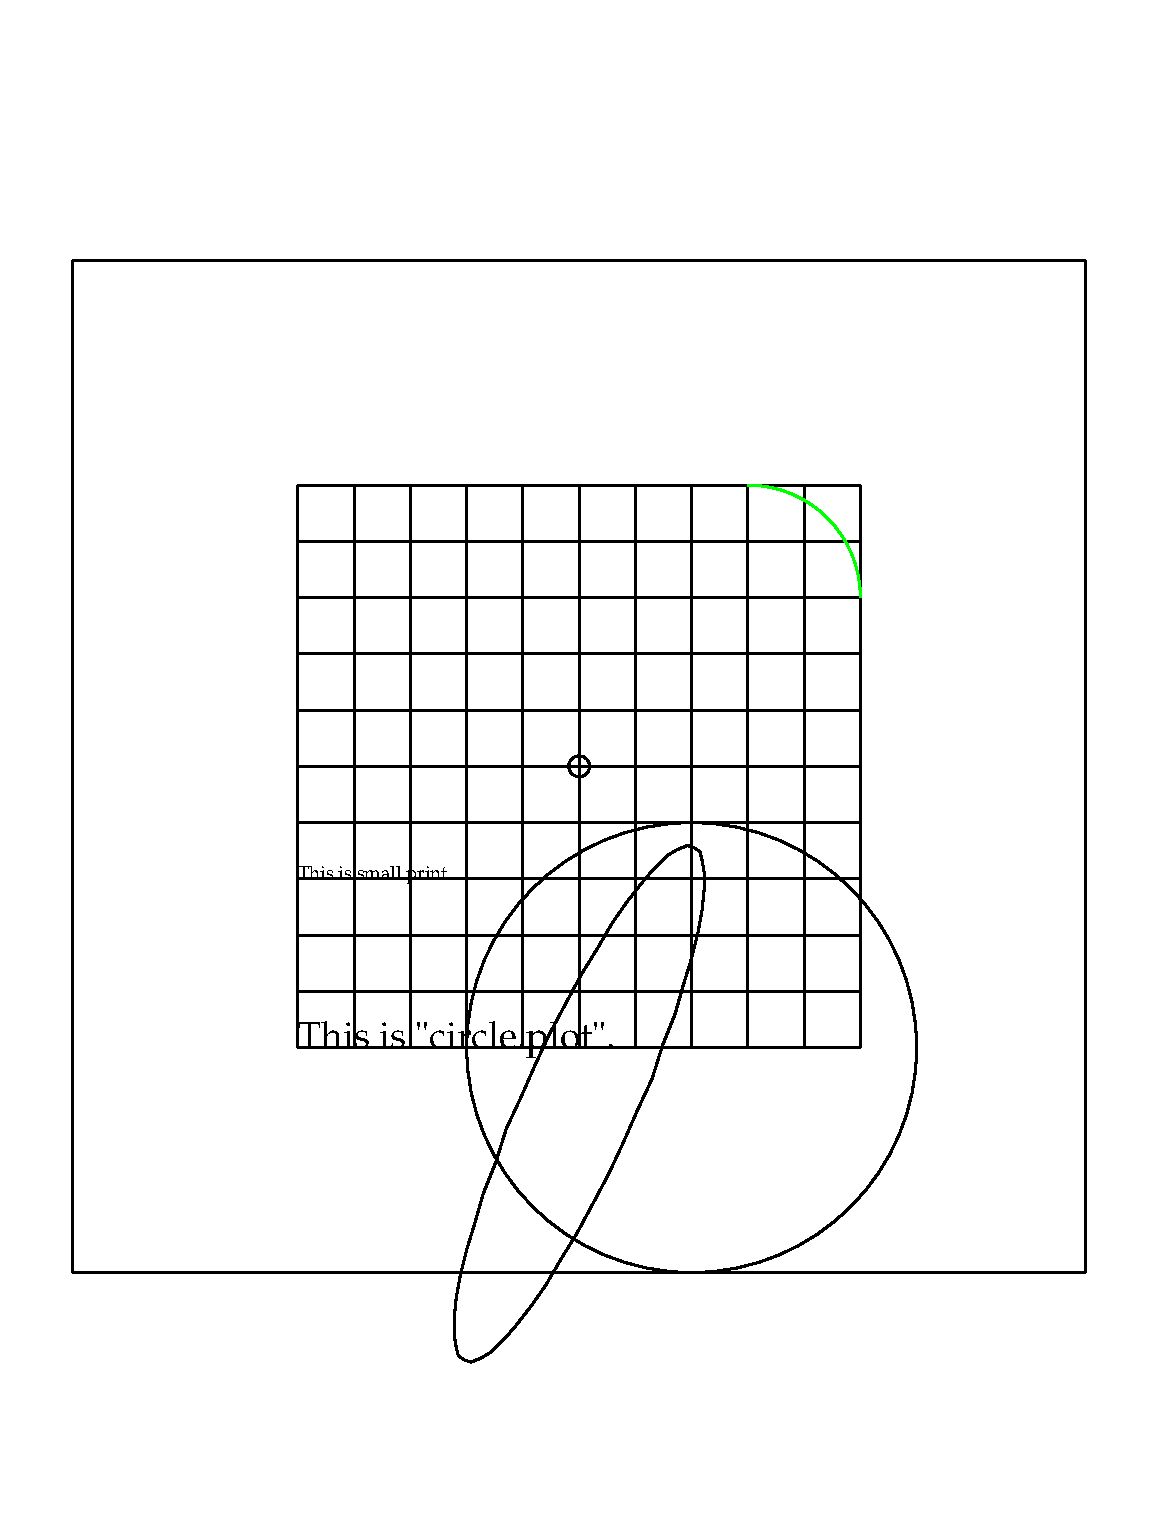
\includegraphics[width=6cm]{./fig/circle.eps}
	\caption{epsSample\cite{EPSFiles}}
	\label{fig:epsSample}
\end{figure}

\subsection{参考文献/関連図書}
bibtexにて,``junsrt.bst''ファイルを改修しています.
\begin{enumerate}
	\item ``misc'' はURL前に改行することで見やすく
	\item ``mymisc'' にて改行せず詰める
	\item 日付は年のみ表示
	\item ``@bachelorthesis''にて,学士論文に対応
	\item ``Master's thesis'' \zr ``修士論文''
\end{enumerate}

\section{パッケージ追加による対応確認}
\subsection{令和対応}
TeX LiveがVer 2017なので,BXwarekiパッケージ\cite{bxwareki}にて,対応しています.

\begin{enumerate}
	\item ``\textbackslash\textbackslash  today'' \zr \today
	\item ``\textbackslash\textbackslash warekitoday'' \zr \warekitoday
\end{enumerate}

\section{旧字体対応}
OTFパッケージにて,対応しています.
{
	\begin{lstlisting}[language=TeX,caption=旧字体]
\newcommand{\toku}{\UTF{5FB7}}
ほげ \toku ほげ
	\end{lstlisting}

	\newcommand{\toku}{\UTF{5FB7}}
	ほげ \toku ほげ
}

\section{自作命令}
ソースを貼っておくので各自試してください.

\begin{lstlisting}[language=TeX, caption=enumiを丸数字に]
\renewcommand{\labelenumi}{\textcircled{\scriptsize \theenumi}} 
\end{lstlisting}

\begin{enumerate}
	\renewcommand{\labelenumi}{\textcircled{\scriptsize \theenumi}} % enumiを丸数字に
	\item hoge1
	\item hoge2
\end{enumerate}

\begin{lstlisting}[language=TeX, caption=丸で文字を加工]
\newcommand{\maruNum}[1]{\textcircled{\scriptsize #1}} 
\end{lstlisting}
{
	\newcommand{\maruNum}[1]{\textcircled{\scriptsize #1}} % 丸で文字を加工
	\maruNum{10} \maruNum{22}
}

\begin{lstlisting}[language=TeX, caption=縦省略記号]
\newcommand{\shoryaku}{\reflectbox{\rotatebox{270}{$\sim$}}} 
\end{lstlisting}
{
	\newcommand{\shoryaku}{\reflectbox{\rotatebox{270}{$\sim$}}} % 省略記号 
	図1 
	\shoryaku \\
	図2
}

\begin{lstlisting}[language=TeX, caption=横省略記号]
\newcommand{\kara}{$\sim$} 
\end{lstlisting}
{
	\newcommand{\kara}{$\sim$} % A〜B
	A \kara Z
}	


\bibliography{bibtex} % 参考文献
\bibliographystyle{junsrt}

\end{document}
